% $Header$

\documentclass{beamer}

% This file is a solution template for:

% - Giving a talk on some subject.
% - The talk is between 15min and 45min long.
% - Style is ornate.



% Copyright 2004 by Till Tantau <tantau@users.sourceforge.net>.
%
% In principle, this file can be redistributed and/or modified under
% the terms of the GNU Public License, version 2.
%
% However, this file is supposed to be a template to be modified
% for your own needs. For this reason, if you use this file as a
% template and not specifically distribute it as part of a another
% package/program, I grant the extra permission to freely copy and
% modify this file as you see fit and even to delete this copyright
% notice. 


\mode<presentation>
{
  %\usetheme{Warsaw}
  %\usetheme{Berlin}
  %\usetheme{metropolis}
  \usetheme{PaloAlto}
  %\usetheme{CambridgeUS}
  %\usetheme{Berkeley}
  
  % font themes
  \usefonttheme{serif}
  %\usefonttheme{structurebold}

  % color themes
  %\usecolortheme{albatross}
  %\usecolortheme{beetle}
  %\usecolortheme{crane}
  %\usecolortheme{dove}
  %\usecolortheme{fly}
  %\usecolortheme{monarca}
  %\usecolortheme{seagull}
  %\usecolortheme{beaver}
  % color themes
  % or ...

  %\setbeamercovered{transparent}
  \setbeamercovered{transparent=5}
  % or whatever (possibly just delete it)
}


\usepackage[english]{babel}
% Place figures exactly where you mean to
%https://tex.stackexchange.com/a/8633/64425
\usepackage{float}
% Place figures exactly where you mean to
% or whatever

\usepackage[utf8]{inputenc}
% or whatever

\usepackage[T1]{fontenc}
% Or whatever. Note that the encoding and the font should match. If T1
% does not look nice, try deleting the line with the fontenc.

% math
\usepackage{amsmath}
\usepackage{amssymb}
\usepackage{amsthm}
% math

% tikz
\usepackage{tikz}
\usetikzlibrary{arrows.meta}
\usetikzlibrary{calc}
% tikz
\usepackage{caption}
\usepackage{hyperref}
\hypersetup{
    colorlinks,
    linkcolor={magenta!50!black},
    citecolor={blue!50!black},
    urlcolor={blue!80!black}
}
% large commented sections
\usepackage{comment}
% large commented sections

% some beautiful fonts
\usepackage{yfonts}
% some beautiful fonts

% canceling in equations
\usepackage{cancel}
% canceling in equations

\title[Infinitesimal Calculus] % (optional, use only with long paper titles)
{Elementary Calculus--An Infinitesimal Approach, Chapters 01, 02}

\subtitle
{Calculus Based on Nonstandard Analysis} % (optional)

\author[JK,KM] % (optional, use only with lots of authors)
{Jerome Keisler\inst{1}}
% - Use the \inst{?} command only if the authors have different
%   affiliation.

\institute[Unknown] % (optional, but mostly needed)
{
  \inst{1}%
  Original Author
}
% - Use the \inst command only if there are several affiliations.
% - Keep it simple, no one is interested in your street address.

\date[September 2025] % (optional)
{September 2025 / Free Learner's School Conversations}

\subject{Fun Conversations at Home School}
% This is only inserted into the PDF information catalog. Can be left
% out. 



% If you have a file called "university-logo-filename.xxx", where xxx
% is a graphic format that can be processed by latex or pdflatex,
% resp., then you can add a logo as follows:

% \pgfdeclareimage[height=0.5cm]{university-logo}{university-logo-filename}
% \logo{\pgfuseimage{university-logo}}



% Delete this, if you do not want the table of contents to pop up at
% the beginning of each subsection:
\AtBeginSubsection[]
{
  \begin{frame}<beamer>{Outline}
    \tableofcontents[currentsection,currentsubsection]
  \end{frame}
}


% If you wish to uncover everything in a step-wise fashion, uncomment
% the following command: 

%\beamerdefaultoverlayspecification{<+->}


\begin{document}

\begin{frame}
  \titlepage
\end{frame}

\begin{frame}{Outline}
  \tableofcontents
  % You might wish to add the option [pausesections]
\end{frame}


% Since this a solution template for a generic talk, very little can
% be said about how it should be structured. However, the talk length
% of between 15min and 45min and the theme suggest that you stick to
% the following rules:  

% - Exactly two or three sections (other than the summary).
% - At *most* three subsections per section.
% - Talk about 30s to 2min per frame. So there should be between about
%   15 and 30 frames, all told.

% [Kedar] I am keeping this structure, but abusing it to serve my purpose.
% [Kedar] I expect this `presentation' to have many hundred slides, if I end up doing it right.
% [Kedar] There are three sections per presentation, no subsections, but each section may have many, many slides. Let's see. I am just getting started with LaTeX and Beamer.
% [Kedar] I may roughly make a chapter in his book a section in this presentation.
\section{Introduction}
\begin{frame}
\frametitle{Introductory Calculus--Infinitesimal Approach}
\framesubtitle{Introducing Infinitesimals}
\label{slide:intro-01}
\begin{itemize}
\item These Are My Notes from H. Jerome Keisler's Book by The Same Name.
\pause\item While Teaching Elementary Calculus to My Daughter, I Realized That I Better Learn The Infinitesimal Approach Better.
\end{itemize}
\end{frame}

\section{Chapter 1}
\begin{frame}
\frametitle{Introductory Calculus--Infinitesimal Approach}
\framesubtitle{1.4 Slope And Velocity; The Hyperreal Line 02}
\label{slide:1.4-02}
\begin{itemize}
\item Consider Two Points \alert{on The Parabola $y=x^2$}: $x_0,y_0$, $x_0+\Delta x, y_0+\Delta y$. 
\pause\item Its \alert{Average Slope between These Points} Is Calculated as \alert{The Slope of The \textit{Secant}}: $\frac{\Delta y}{\Delta x}=\frac{(x_0+\Delta x)^2-(x_0)^2}{\Delta x}=2x_0+\Delta x$.
\pause\item This Computation Makes Sense \alert{Only When $\Delta x\ne 0$} Because \alert{Otherwise $\frac{\Delta y}{\Delta x}$ Is Undefined}.
\pause\item \alert{Intuitively, If Non Rigorously,} We \alert{Consider $\Delta x$ Negligible}.
\pause\item We Therefore State That \alert{The Average Slope Equals $2x_0$}.
\end{itemize}
\end{frame}

\begin{frame}
\frametitle{Introductory Calculus--Infinitesimal Approach}
\framesubtitle{1.4 Slope And Velocity; The Hyperreal Line 02}
\label{slide:1.4-02}
\begin{itemize}
\item \begin{figure}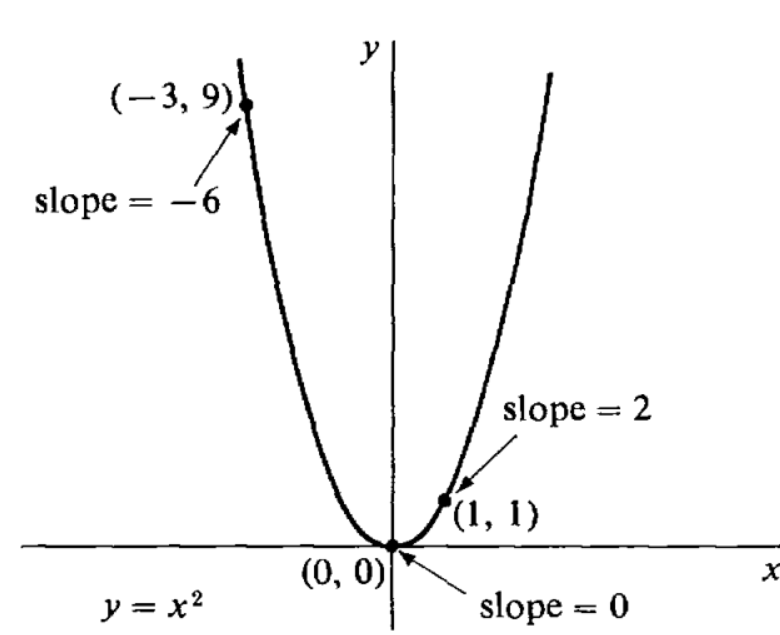
\includegraphics[width=.5\textwidth]{images/slope-examples-parabola}\end{figure}
\pause\item For Example, The Slope Is $2x_0=2\cdot 0=0$ at $(0,0)$, $2\cdot 1=2$ at $(1,1)$, And $2\cdot -3=-6$ at $(-3, 9)$.
\end{itemize}
\end{frame}

\begin{frame}
\frametitle{Introductory Calculus--Infinitesimal Approach}
\framesubtitle{1.4 Slope And Velocity; The Hyperreal Line 03}
\label{slide:1.4-03}
\begin{itemize}
\item We Can Visualize \alert{Slope as Velocity}.
\pause\item If The Horizontal Axis Represents Time And Vertical Axis Position, Is \alert{The Average Velocity between $(y_0,t_0)$ and $(y_0+\Delta y, t_0+\Delta t)$} = \alert{The Velocity \textit{at\footnote{In Physics, We Call It The \textit{Instantaneous Velocity}.}} Either} of Those Points?  
\pause\item Since in This Case The Velocity Constantly Increases, The Answer Is \alert{NO}.
\pause\item $v_{ave}=2t_0+\Delta t$ And, \alert{After We Treat $\Delta t$ Negligible}, $v_{ave}=2t_0$. 
\end{itemize}
\end{frame}

\begin{frame}
\frametitle{Introductory Calculus--Infinitesimal Approach}
\framesubtitle{1.4 Slope And Velocity; The \alert{Trouble with Intuition}}
\label{slide:1.4-04}
\begin{itemize}
\item In Either Case (Slope, Velocity), The Intuitive Reasoning Fails to Clarify \alert{When Something Is to Be Treated Negligible}.
\pause\item We Need a \alert{Sharp Distinction} between \alert{Which Numbers Are Small Enough to Ignore And Which Aren't}.
\pause\item Actually, \alert{No \underline{Real Number} Except $0$ Is Small Enough To Ignore\footnote{Does This Hint at a New \textit{Kind} of Number?}}.
\pause\item To Address This Difficulty, We \alert{Take The Bold Step\footnote{A Rigorous Treatment Is Provided by Keisler in His \textit{Foundations}.} of Introducing a New \textit{Kind\footnote{Unreal?} of Number}} Which Is \alert{Infinitely Small And Yet $\ne 0$}.
\end{itemize}
\end{frame}

\begin{frame}
\frametitle{Introductory Calculus--Infinitesimal Approach}
\framesubtitle{1.4 Properties of Infinitesimals}
\label{slide:1.4-05}
\begin{definition}[Infinitely Small Or Infinitesimal Number]
A \textit{Number} $\varepsilon$ Is Said to Be \textit{Infinitely Small, Or Infinitesimal,} If $-a<\varepsilon<a \quad\forall a\in\mathbb{R}^+$.
\end{definition}
\begin{itemize}
\item Note: All Infinitesimal Numbers Exist Between \textit{Every} Positive Real Number And Its Negative\footnote{M. Gardner Calls It The \textit{Number Neverland.}}.
\pause\item The \alert{Only \underline{Real} Infinitesimal Number is $0$}.
\pause\item We Introduce A New Number System, \alert{The Hyperreal Numbers}, Which \alert{Contains All The Real Numbers And \underline{Infinitesimals That Are Not Zero}}.
\pause\item \alert{Integers Create Rationals. Rationals Create Reals. Reals Create Hyperreals.}
\pause\item Right Now, \alert{We Study Properties of Hyperreals Needed for The Calculus}. We'll Study Their Creation Later.
\end{itemize}
\end{frame}

\begin{frame}
\frametitle{Introductory Calculus--Infinitesimal Approach}
\framesubtitle{1.4 Properties of Hyperreals And Infinitesimals}
\label{slide:1.4-06}
\begin{itemize}
\item $\mathbb{R}^*$: The Set of All Hyperreal Numbers.
\pause\item $x\in\mathbb{R}\implies x\in\mathbb{R}^*\implies\mathbb{R}\subseteq\mathbb{R}^*$. However, $\mathbb{R}^*$ Has Other Elements Too, \alert{$\therefore \mathbb{R}\subset\mathbb{R}^*$}.
\pause\item Infinitesimals in $\mathbb{R}^*$ Are of \alert{Three Kinds: Positive, Negative, And \underline{The Real Number $0$}}.
\pause\item $x,x_0,x_1,y,\dots$ Denote Reals. $\Delta x, \Delta y, \varepsilon\text{ (epsilon)},\delta\text{ (delta)},\dots$ Denote Infinitesimals.
\pause\item If $a,b\in\mathbb{R}^*$ And $a-b \text{ Is Infinitesimal}$, Then We Say \alert{$a$ Is ``Infinitely Close'' to $b$}.
\begin{itemize}
\pause\item If $\Delta x=(x_0+\Delta x)-(x_0)$ Is Infinitesimal, Then \alert{$x_0+\Delta x$ And $x_0$ Are ``Infinitely Close'' to Each Other}.
\end{itemize}
\pause \item If \alert{$\varepsilon$ Is Positive Infinitesimal}, Then 
\begin{itemize}
\pause\item\alert{$-\varepsilon$ Is Negative Infinitesimal}.
\pause\item\alert{$\frac{1}{\varepsilon}$ Is Infinite Positive, > All Real Numbers}.
\pause\item\alert{$\frac{-1}{\varepsilon}$ Is Infinite Negative, < All Real Numbers}.
\end{itemize}
\end{itemize}
\end{frame}

\begin{frame}
\frametitle{Introductory Calculus--Infinitesimal Approach}
\framesubtitle{1.4 More Properties of Hyperreals And Infinitesimals}
\label{slide:1.4-07}
\begin{itemize}
\item<1->
Hyperreal Numbers Which Are Not Infinite, Are \alert{Finite Numbers}.
\item<2->
About each $c\in\mathbb{R}$ Is \alert{A Portion of Hyperreal Line Composed of The Numbers Infinitely Close to $c$}.
\visible<2->
{
\begin{figure}[H]
\centering
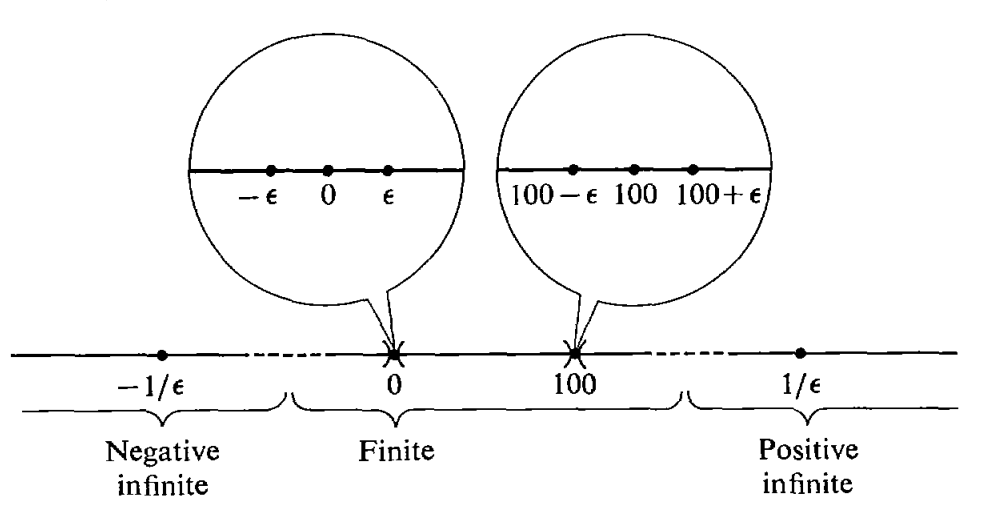
\includegraphics[width=.5\textwidth]{images/infinitesimal-microscope}
\caption{Finite And Infinite Parts of The Hyperreal Line (\textit{Infinitesimal Microscope} about $c=0,c=100$)}
\label{fig:finfinhyperreal}
\end{figure}
}
\item<3->
\alert{Numbers Infinitely Close to $0$ Are Infinitesimals}.
\end{itemize}
\end{frame}

\begin{frame}
\frametitle{Introductory Calculus--Infinitesimal Approach}
\framesubtitle{1.4 Startling Observation about \alert{The Physical Space}}
\label{slide:1.4-08}
\begin{block}{The Nature of Physical Space}
Euclid Struggled to Define \alert{a `Point': Something That Has a Position But No Magnitude\footnote{Isn't This `Definition' (\textit{Accepted} for Centuries) \textit{Meaningless}?}}.

We Have No Way of Knowing What a Line in Physical Space Is Really Like (``What Is It Composed of?''). It Might Be Like the Hyperreal Line (with Infinitesimals Surrounding Every `Real Point'), The Real Line (without Any Infinitesimals), Or Neither. \alert{However, in Applications of The Calculus It Is Helpful to Imagine a Line in Physical Space as A Hyperreal (Rather Than Real) Line. The Hyperreal Line Is, Like The Real Line, A Useful \underline{Mathematical Model}\footnote{And, Here's A Stark Reminder: All Models Are Wrong; Some Are Useful!} for A Line in Physical Space.}
\end{block}
\end{frame}

\begin{frame}
\frametitle{Introductory Calculus--Infinitesimal Approach}
\framesubtitle{1.4 Defining Slope w Infinitesimals}
\label{slide:1.4-09}
\begin{definition}[The \alert{Slope of A Curve at $(x_0,y_0)$}]

Let $y=f(x)$ Be a Certain Function. Let $P(x_0,y_0)$ Be Any Point on The Curve Representing $y$. \alert{Let $\Delta x$ Be a Positive Or Negative Infinitesimal}. Consider A Point $(x_0+\Delta x,y_0+\Delta y)$ \alert{Infinitely Close to P}.

Then,

\[
\text{Slope of $f$ at} (x_0,y_0)=\text{\alert{Real Number Infinitely Close to }} \frac{\Delta y}{\Delta x}
\]
\label{def:slope}
\end{definition}
Note: The Slope is \textit{Defined to Be} A Real Number.
\end{frame}

\begin{frame}
\frametitle{Introductory Calculus--Infinitesimal Approach}
\framesubtitle{1.4 Calculating Slopes with Infinitesimals: Examples}
\label{slide:1.4-10}
\begin{example}[Slope of $y=x^2$]
The Definition [\ref{def:slope}] Defines Slope as \alert{The Real Number Infinitely Close to $\frac{\Delta y}{\Delta x}$}.

\begin{equation}
\begin{aligned}
y+\Delta y &= (x+\Delta x)^2  \\
\therefore \Delta y &= 2x\Delta x+(\Delta x)^2 \\
\therefore \frac{\Delta y}{\Delta x} &= 2x+\Delta x \\
\therefore \text{Slope}&=2x \;\text{(From Definition [\ref{def:slope}])}
\end{aligned}
\label{eq:slope-of-y=x^2}
\end{equation}
\pause
$2x$ Is the \alert{Real Number Infinitely Close to The Hyperreal Number $2x+\Delta x$}.
\end{example}
\pause
In This Example It Was Rather Straightforward to Show $2x+\Delta x$ And $2x$ Are Infinitely Close To Each Other. 
\end{frame}

\begin{frame}
\frametitle{Introductory Calculus--Infinitesimal Approach}
\framesubtitle{1.4 Calculating Slopes with Infinitesimals: Examples}
\label{slide:1.4-11}
\begin{example}[Slope of $y=x^3$]
The Definition [\ref{def:slope}] Defines Slope as \alert{The Real Number Infinitely Close to $\frac{\Delta y}{\Delta x}$}.

\begin{equation}
\begin{aligned}
y+\Delta y &= (x+\Delta x)^3  \\
\therefore \Delta y &= \cancel{x^3}+3x^2\Delta x+3x(\Delta x)^2+(\Delta x)^3-\cancel{x^3}\\
\therefore \frac{\Delta y}{\Delta x} &= 3x^2+3x\Delta x+(\Delta x)^2 \\
\end{aligned}
\label{eq:slope-of-y=x^3}
\end{equation}
If (Because $\Delta x$ Is Infinitesimal), $3x\Delta x+(\Delta x)^2$ Is Infinitesimal, Then 
\begin{equation}
\begin{aligned}
\text{Slope}&=3x^2
\end{aligned}
\end{equation}
\end{example}
\end{frame}

\begin{frame}
\frametitle{Introductory Calculus--Infinitesimal Approach}
\framesubtitle{1.4 Which Hyperreal Numbers Are Infinitely Close to Each Other?}
\label{slide:1.4-12}
\begin{itemize}
\item
\alert{$\Delta x$ Is An Infinitesimal. That Brings $x+\Delta x$ Infinitely Close to $x$.}

\pause \item However, It Is Not Immediately Clear That $3x^2+3x\Delta x+(\Delta x)^2$ Is Infinitely Close to $3x^2$, Is It?
\pause \item It Depends on Whether $3x\Delta x+(\Delta x)^2$ Is Infinitesimal. We Only Know $\Delta x$ to Be Infinitesimal. Does That Make $3x^2+3x\Delta x+(\Delta x)^2$ Infinitesimal?

\pause\item Thus, Unless We Have Precise Rules To Determine Which Hyperreal Numbers Are \alert{Infinitely Close} to Which Real Numbers, We Won't Be Able to Go Too Far.
\end{itemize}
\pause
\alert{That's What We Study Next}.
\end{frame}

\section{Chapter 2}
\section{Summary}

\end{document}


